Nach sorgfältiger Recherche über aktuelle Lösungen bezüglich der Integration von verschiedenen Systemen, sind wir auf das Open Integration Hub (OIH) gestoßen.
Das OIH ist ein Open Source Framework, das verschiedene Ressourcen bündeln und zentral zur Verfügung stellen kann \footnote{Siehe https://www.openintegrationhub.org}. Dabei ist das Ziel des OIH, einen standardisierten Datenaustausch zwischen verschiedenen Geschäftsanwendungen zu ermöglichen. Dies wird durch eine flexible Microservice-Architektur erreicht, in der verschiedenen Schnittstellen schnell und mit wenig Aufwand an das Framework angebunden werden können, sodass der Entwicklungs- und Wartungsaufwand erheblich reduziert wird. Bei der Konzeption des OIH wurde viel Wert auf Skalierung und Flexibilität gelegt, weshalb sie auf modernen Cloud-Technologien, wie Docker Containern und einem Kubernetes Cluster aufsetzt. Dadurch können verschiedene Services dynamisch in der Cloud je nach Bedarf bereitgestellt werden, welche über ein externes messaging system beziehungsweise event bus (RabbitMQ) miteinander kommunizieren und lose gekoppelt sind. Die Tabelle \ref{tab:Essentielle Services im OIH} listet die essentiellen Services mit ihren Funktionen auf.


\begin{longtable}{|c|p{8,5cm} |} \hline
\textbf{Service} & \textbf{Beschreibung}\\ \hline \bottomrule
Identity Access Management & •	Sorgt für eine sichere Authentifizierung und Autorisierung von Benutzern/Kunden \newline • Benutzer- und Rollenverwaltung, Audit-Logging \\ \hline
Component Repository & • Speicherung von Informationen über Integration Components \newline  • Bereitstellung der Informationen über gespeicherte Integration Components für andere Services \\ \hline
Component Orchestrator & •	Verantwortlich für das Deployment von Integration Flows und für eine faire Ressourcenverteilung (z.B. CPU, Arbeitsspeicher, Netzwerkressourcen) im OIH
\newline •	Sicherstellung, dass die entsprechenden Integration Flows je nach Konfiguration skaliert werden
\newline •	Sicherstellung, dass Integration Flows nicht mehrfach ausgeführt werden
\newline •	Verhinderung von „Over-scheduling“ im OIH
\newline •	Redeployment von Integration Flows, wenn diese veraltet sind \\ \hline
Flow Repository & •	Speicherung, Abrufung, Aktualisierung und Löschung von Integration Flows
\newline •	Startet und stoppt vorhandene Integration Flows \\ \hline
Data Hub (optional) & •	Zuständig für die Speicherung, den Abruf und Bearbeitung von Datensätzen im OIH, die aus den Drittsystemen kommen
\newline •	Dient als zentraler Datenspeicher für synchronisierte Daten \\ \hline
Dispatcher Service & •	Ist zuständig für das Routen von Nachrichten zwischen individuellen Connector Flows auf Basis vom Benutzer definierten Konfigurationen
\newline •	Dient für den zentralen Datenaustausch in einem Hub \& Spoke model \\ \hline
Scheduler & •	Ist zuständig für die periodische Ausführung von Integration Flows \\ \hline
Webhooks (optional) & •	Ermöglicht die Konfiguration von Webhooks, sodass beim Einkommen von http-Aufrufen (beispielsweise von externen Systemen) bestimmte Actions (z.B. Abruf von neuen Daten aus dem Drittsystem) ausgeführt werden können \\ \hline
Secret Service & •	Speichert und verwaltet die Client-/User-Zugangsdaten für externe Systeme \\ \hline
Meta Data Repository & •	Zuständig für die Speicherung von domain und master data models, die für die Datenvalidierung bezüglich dem Transforming/Mapping in das standardisierte Format des OIH genutzt werden \\ \hline
Integration Layer Service (ILS) & •	Empfängt Datenobjekte von einem oder mehreren Integration Flows und führt gegen das Objekt Geschäftslogik (merge/split) aus und validiert anschließend das Ergebnis gegen das bereitgestellte Schema oder einem Schema aus dem Meta Data Repository.
\newline •	Temporäre Datenhaltung für die Verarbeitung und Validierung von Daten für verschiedene Integration Flows
\newline •	Stellt REST API zur Verfügung, um neue Objekte zu speichern und abzurufen \\ \hline
Smart Data Framework Adapter (SDF) & •	Ermöglicht die Kommunikation mit dem Smart Data Framework (bestehend z.B. aus Integration Layer Service, Data Hub, Dispatcher, Flow Repository, Component Orchestrator, Meta Data Repository)
\newline •	Leitet einkommende Events zum Smart Data Framework weiter, sodass diese von nachfolgenden Integration Components bearbeitet werden können \\ \hline
\caption{Essentielle Services im OIH}
\label{tab:Essentielle Services im OIH}
\end{longtable}

Zudem sind weitere Services (z.B. logging, auditing, conflict management etc.) im OIH verfügbar, die für den Betrieb optional sind.\footnote{Siehe https://openintegrationhub.github.io/docs/Services/Services.html}
Das Grundprinzip des OIHs ist es, dass ein Anwender verschiedene Integration Flows erstellen kann, die verschiedene Integration Components (Adapter/Transformer) deployen und starten können. Diese Integregation Flows enthalten Actions/Triggers für die Integration Components, um Daten aus Drittsystemen abzufragen, zu transformieren und in anderen Systemen zu speichern. Dabei können Integration Flows in einem bestimmten Zeitintervall gestartet oder über Webhooks ausgeführt werden. Weiterhin können die Integration Flows und Integration Components beliebig miteinander orchestriert werden, sodass Komponenten sehr gut wiederverwendet können und eine hohe Skalierung erreicht wird. Bei Bedarf können die Daten für eine Domäne weiterhin in einem zentralen Datahub über eine MongoDB aufbewahrt werden, um die Daten standardisiert für andere Anwendungen bereitzustellen. \\
Die Abbildung \ref{fig:Architektur des OIH mit essentiellen Services} zeigt die Architektur des OIH mit den essentiellen Services.

\begin{figure}[!h]
\centering
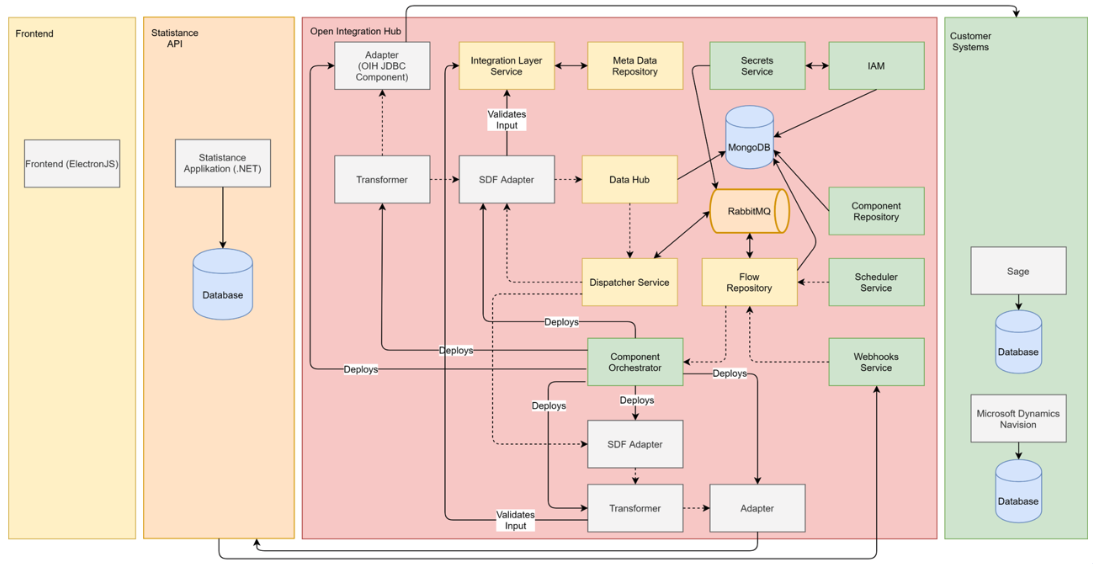
\includegraphics[width=15cm]{images/0x_implementation_possibilities/opt3.png}
\caption{Architektur des OIH mit essentiellen Services}
\label{fig:Architektur des OIH mit essentiellen Services}
\end{figure}

Der Vorteil hierbei wäre gewesen, dass lediglich neue Integration Components (Adapter/Transformer) mit Java oder JavaScript entwickelt/beschafft hätte werden müssen, um neue Drittsysteme anzubinden. Somit hätte sich bei dieser Lösung eine enorme Reduzierung des Entwicklungs- und Wartungsaufwands ergeben, da das OIH bereits eine Struktur/Schnittstelle über parent images/libraries vorgibt, um neue Komponenten in der Plattform zu integrieren. Nachdem die Integration Components vorhanden gewesen wären, hätte Statistance lediglich Integration Flows (gegebenfalls über das bereits vorhandene User Interface) erstellen müssen, die die Components verwenden hätten, um die Daten aus den Drittsystemen abzuholen beziehungsweise zu speichern. Die Anbindung der eigenen Applikation an das OIH hätte Statistance ohne viel Aufwand über Adapter (z.B. REST API) erreicht. Anschließend hätte Statistance Integration Flows über bereitgestellte Schnittstellen der Scheduler/Webhooks-Services ausführen können. Ein weiterer Vorteil wäre zudem gewesen, dass es kommerzielle Lösungen (z.B. elastic.io, flowground) gibt, die auf dem OIH basieren, und bereits zahlreiche kommerzielle Konnektoren (Adapter/Transformer) von den Anbietern angeboten werden \footnote{Siehe https://www.elastic.io/connectors/}. Dementsprechend wäre eine gewisse Qualität der Lösung und Support von den Firmen zu erwarten gewesen. Ansonsten gibt es auch eine Community, die neue Konnektoren entwickelt und diese öffentlich zugänglich macht. Allgemein ist das OIH von einer hohen Standardisierung geprägt, welches eine einfache Integration zwischen verschiedenen Systemen ermöglicht und dabei sehr flexibel und skalierbar ist. \\
Obwohl das OIH leicht erweiterbar ist, gab es allerdings auch einige Nachteile. Zum einem erfordert das OIH eine gewisse Einarbeitungszeit, falls vom Standard abgewichen wird und Anpassungen gemacht werden müssen, da das Framework insgesamt sehr komplex und umfangreich ist. Demzufolge wäre auch ein relativ hoher Aufwand beim Betrieb zu erwarten gewesen, zumal eine relativ hohe Anzahl an Services im OIH überwacht und gepflegt werden müssen. Zum anderen basiert das OIH auf Cloud-Technologien (Docker/Kubernetes), die zwar in der Cloud als auch On-Premise genutzt werden können, jedoch ebenfalls ein gewisses Knowhow beim Betrieb voraussetzten. Hinzu kam, dass das Open-Source-Projekt noch nicht wirklich populär ist\footnote{Siehe https://github.com/openintegrationhub} und die OIH Community noch nicht sehr stark ist, sodass Fehlerbehebungen dort größtenteils selbst hätte durchgeführt werden müssen. Schlussendlich fallen für den Betrieb des OIH auch höhere Kosten für die Infrastruktur an, da hierfür mehr Hardware-Ressourcen für die Services bereitgestellt werden müssen. Die Tabelle \ref{tab:Beispielhafte Preiskalkulation für das OIH in der GKE} zeigt eine beispielhafte Preiskalkulation für den Betrieb des OIH in der Google Kubernetes Engine (GKE) Clusters mit zwei Worker Nodes innerhalb der Google Cloud Platform.

\begin{table}[h!]
\begin{tabular}{|c|p{3cm} |}
\hline
\textbf{Komponente} & \textbf{Preis in EUR}\\ \hline \bottomrule
2x Worker Nodes (n1-standard-2, 7,5 GBs, 2vCPUs, 1 Jahr Commitment) & 101,24 \\ \hline
1x Load Balanacer (10 Forwarding Rules, Netzwerk ingress 10 GB traffic) & 59,23 \\ \hline
1x Standard Provisioned Persistent Disk (100 GB) & 4,32 \\ \hline
Gesamtpreis pro Monat & 164,79 \\ \hline
\end{tabular}
\caption{Beispielhafte Preiskalkulation für das OIH in der GKE}
\label{tab:Beispielhafte Preiskalkulation für das OIH in der GKE}
\end{table}